\section{Introduction}

Contemporary security identification has led to a plethora of biometric-based authentication systems. From palm readers at testing centers to facial recognition on smartphones, many systems are now used to regularly verify identities. These inherence-based systems are attractive in comparison to knowledge or possession-based methods of authentication because biometrics are unique, unforgettable, and far more difficult to steal than a password or swipe card.

Although biometric identification appears sophisticated when compared to something like physical keys, it does not come without its own share of caveats. For example, owing to the ongoing Covid19 pandemic, many people wear masks when outside of their house, challenging most facial recognition systems. Additionally, biometrics that rely on touch, such as fingerprinting, raise safety concerns, as the scanner may become a vector for virus transmission. Despite these setbacks, given their merits and widespread deployment, biometric identification systems are unlikely to disappear.

One behavioral biometric that has gained recent success and is worth further consideration given current constraints is gait recognition. Usage of gait recognition has grown in the security industry in recent decades due to advances in deep learning. Singh et al. \cite{Singh2019APerspectives} categorized gait recognition into two main categories, vision-based and sensor-based. In vision-based approaches, cameras capture data of a person walking for the purpose of gait recognition. Sensor-based gait recognition is performed using either wearable sensors which produce kinematic data, or floor sensors which produce kinetic data \cite{Connor2018BiometricFeatures}.


%\section{Datasets}
This project uses two different datasets, UoM-Gait-Dataset and Stepscan. The UoM-Gait-Dataset was obtained from iMAGiMAT sensor \cite{Cantoral-Ceballos2015IntelligentEnvironments} (an optical floor sensor). This sensor contains about 160 distributed \gls{pof} that indicate the foot pressure signals over time. Some studies like \cite{Costilla-Reyes2020DeepHealthcare} used this dataset to construct images for their research.

The second dataset that was used for this project is called the Stepscan dataset \cite{Connor2015ComparingBiometrics}. This dataset was obtained from high-resolution floor tiles that have recently been introduced by Stepscan Technologies Inc.

Figure \ref{fig:Stepscan_dataset} indicates three frames from this dataset. This dataset consists of a spatial-temporal tensor, X, with dimensions $S \times T \times H \times W$ where $S$ represents the number of samples. $T$ is the number of temporal observations or video frames; $H$ and $W$ are the dimension of the image in pixels. Moreover, both datasets include information on different walking speeds. 

This project aims to find some temporal features from the datasets to construct a classifier for verification purposes. The nature of data in the first dataset is time series, whereas Stepscan is a video-base dataset. There are several methods for converting a tensor (like video) to 2D time-series data. 

Chen et al. in \cite{Chen2006GaitModel} used contour width for defining a one-dimensional signal. They utilized some morphological operations on the background-subtracted silhouette image to extract the outer contour. Afterwards, according to the contour width of each image row, a one-dimensional signal was generated.

Another method could be that the pixel values in each frame are plotted over time. By this means, the $H * W$ time-series will be produced for each sample.

In the final method, some spatial features are extracted from each frame (e.g. centroid and maximum pressure in each image). Afterwards, we track these values over time (next frames). As a result, 3D videos with size $T \times H \times W$ are converted to the four 2D time-series data. Costilla-Reyes et al. utilized this method to combine the output of 160 distributed \gls{pof} \cite{Costilla-Reyes2018DeepSensors}.

In this research, the last mentioned method was applied to produce time-series data. Figure \ref{fig:extracted_features} indicates the time series extracted from the Stepscan dataset. The spatial features extracted in each frame were maximum pressure (figure \ref{fig:extracted_features_max}), the center of pressure (COP) (figures \ref{fig:extracted_features_yCe} and \ref{fig:extracted_features_xCe}), and the average pressure (figure \ref{fig:extracted_features_sum}). 

In general, there are two modes for footprint recognition or generally in the biometric system: verification or identification mode \cite{Jain2004AnRecognition}. In verification mode, the biometric system is used for accessing buildings or data. In other words, the system compares the claimed person with its dataset to determine whether or not the claim is valid. These systems consume less processing power and time \cite{Jain2004AnRecognition}. 

%Because verification systems only need to compare the presented biometric to a biometric reference stored in the system, they can generate results more quickly and are more accurate than identification systems, even when the size of the database increases.

This project will focus on verification. We hope to engineer some temporal features which help us to classify participants. Furthermore, this research will be implemented in Python, and the source codes are available on the GitHub repository \cite{SKazemii/EE6563}.  

The rest of this research is organized as follows: Section 2 provides the relevant works and researches. Then, in Section 3, the time domain features as well as machine learning models are defined. In Section 4, we discuss the results, and we propose future work in Section 5.
%As the figure \ref{fig:Stepscan_dataset} shows the data is a image not a time series data. Therefore, we need to convert our data to a time series. 

\begin{figure}
    \centering
    \begin{minipage}[b]{.5\textwidth}
        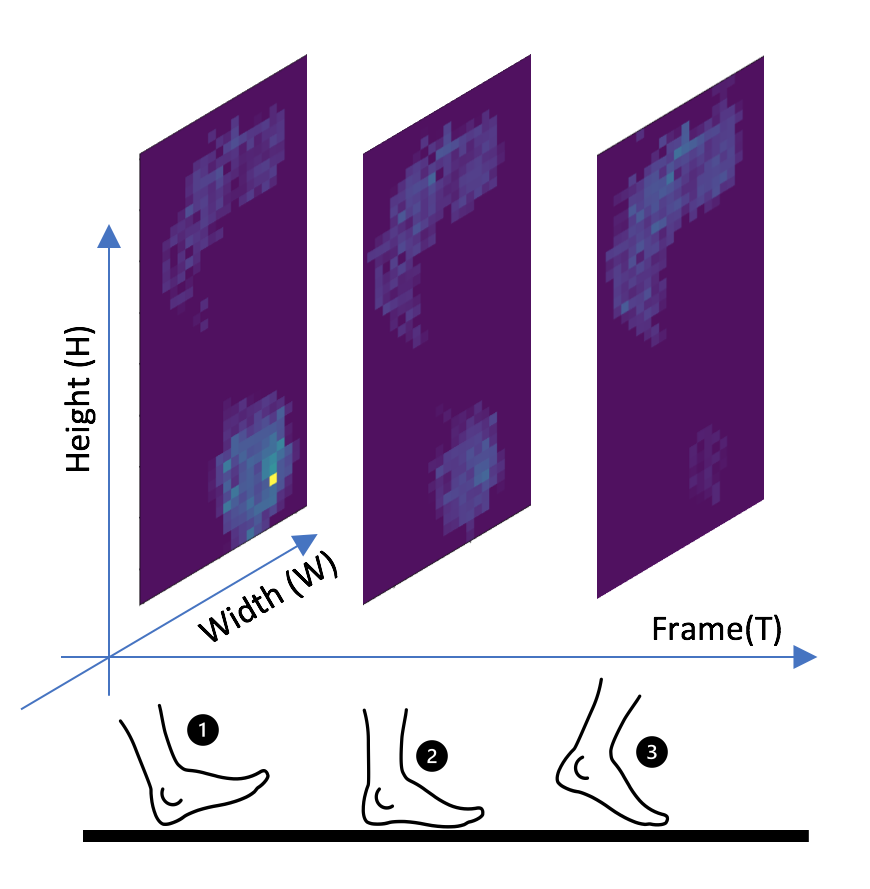
\includegraphics[width=\textwidth]{figures/project/frame2.png}
    \end{minipage}
    \caption{Different frames of footprint video in Stepscan dataset.}
    \label{fig:Stepscan_dataset}
\end{figure}


\begin{figure}
     \centering
     \begin{subfigure}[b]{0.5\textwidth}
         \centering
         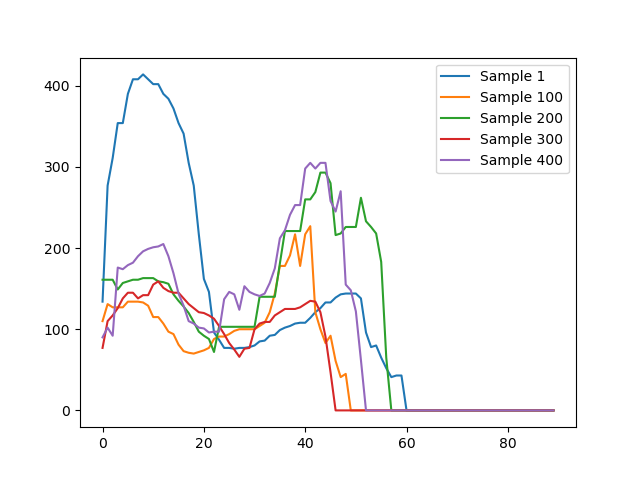
\includegraphics[width=0.9\textwidth]{figures/project/df_max.png}
         \caption{The maximum pressure in each frame}
         \label{fig:extracted_features_max}
     \end{subfigure}
     \hfill
     \begin{subfigure}[b]{0.5\textwidth}
         \centering
         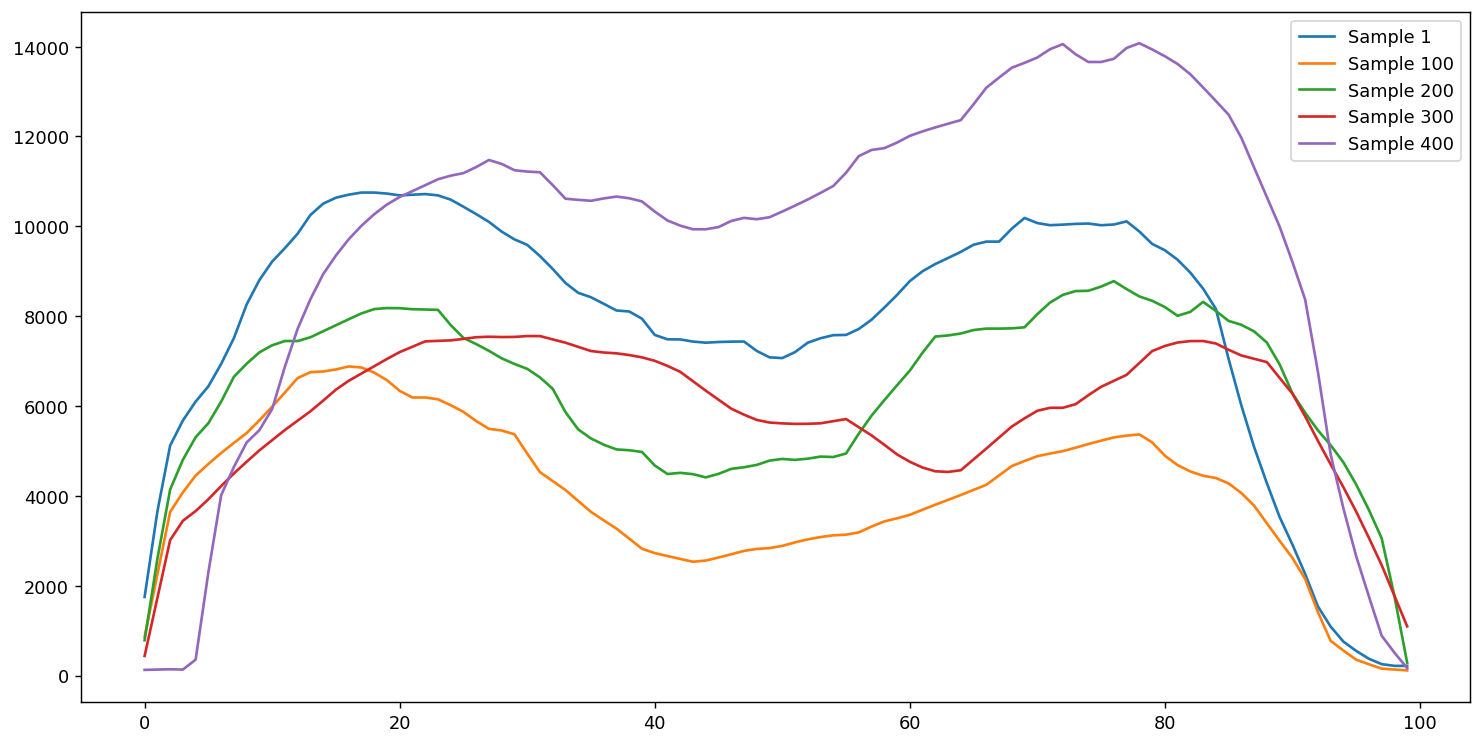
\includegraphics[width=0.9\textwidth]{figures/project/df_sum.png}
         \caption{The average pressure in each frame}
         \label{fig:extracted_features_sum}
     \end{subfigure}
     \vfill
     \begin{subfigure}[b]{0.5\textwidth}
         \centering
         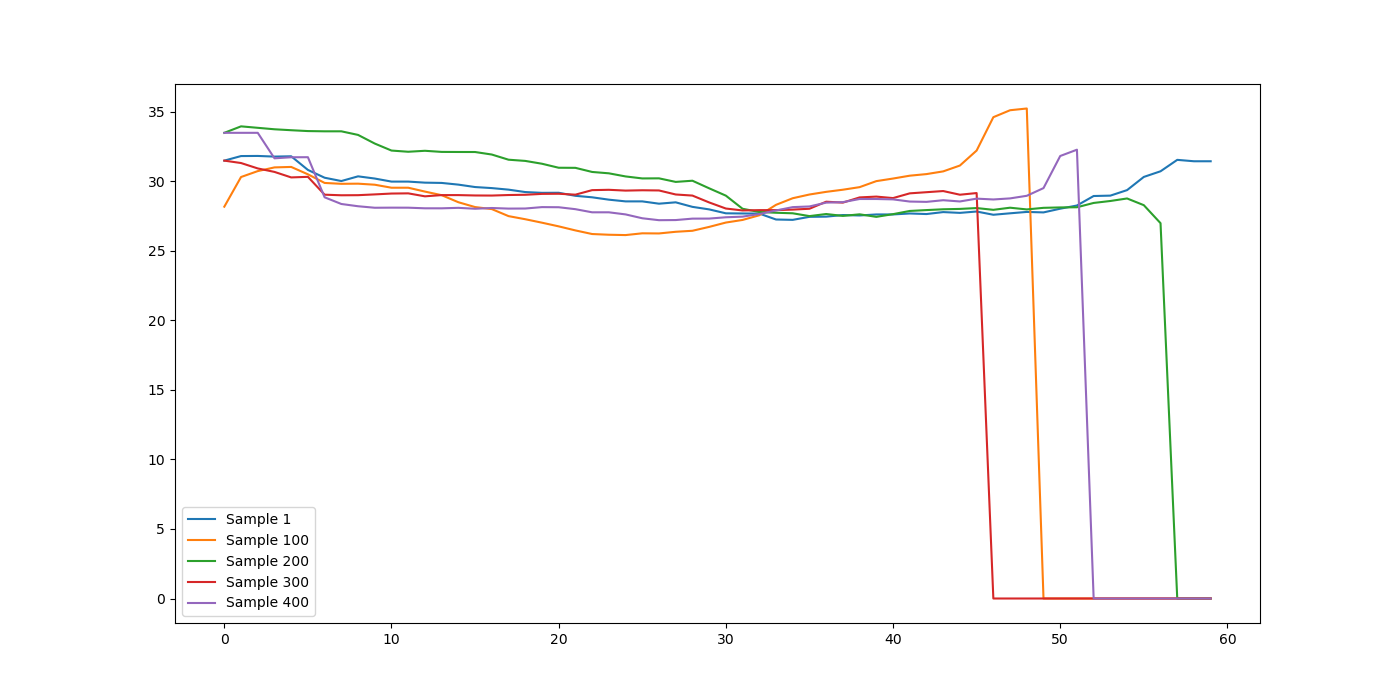
\includegraphics[width=0.9\textwidth]{figures/project/df_xCe.png}
         \caption{The x position in the center of pressure (COP) in each frame}
         \label{fig:extracted_features_xCe}
     \end{subfigure}
     \hfill
     \begin{subfigure}[b]{0.5\textwidth}
         \centering
         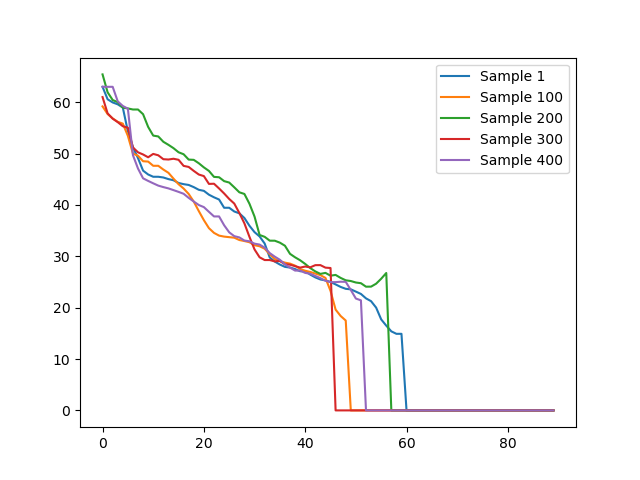
\includegraphics[width=0.9\textwidth]{manuscript/src/figures/project/df_yCe.png}
         \caption{The y position in the center of pressure (COP) in each frame}
         \label{fig:extracted_features_yCe}
     \end{subfigure} 
        \caption{The time series extracted from the Stepscan dataset based on four spatial features. The horizontal axis indicates the frame number.}
        \label{fig:extracted_features}
\end{figure}




